\lab{Unit Testing In Python}{Unit Testing In Python}

%\objective{Convey the importance of unit testing in code, especially in the corporate world. Unit testing in python is easy, valuable, and powerful. Help students understand how to use unit testing to become a more effective and productive programmer.}

\objective{
One of the hardest parts of computer programming is ensuring that a program does what you expect it to do.
For instance, a program may fail to meet specifications, or may work in some cases and not in others.
Finding and fixing errors may be difficult and time consuming, especially if the program is very large or if many people are contributing the same program.
Unit testing is a simple solutions which helps to solve many of these difficulties in programming.
\\ \indent In this lab, we explore unit testing in Python and apply them to the concept of Test Driven Design.
}

A \emph{unit test} is a formal test that checks the smallest testable pieces of a program (often functions or classes) for correctness, independent of the rest of the code.
Testing each unit of code verifies that each piece of code works as expected.
When code does contain bugs, it is easier to identify which part of the code they came from.
Writing unit tests also ensures that the specifications of a program are met.

Unit Testing is especially vital in corporate settings, where many developers often work on the same code or expand existing code.
By keeping a collection of unit tests associated with a program, developers can ensure that when adding new features, they do not break any existing features of the program.

A well written collection of unit tests can ensure that all functions, and by extension an entire program, works correctly.

\section*{PyTest} % ===========================================================

A unit test verifies that a piece of code works by comparing actual output with expected output, given some specific input.
Unit tests are often written for individual functions, but they can also test whole classes or files.

To test a function we use Python's reserved word \li{assert} and provide our function with input and expected output. Basic assert statements take the form

\begin{lstlisting}
assert <truth statement>, "message"
\end{lstlisting}

which raises an \li{AssertionError} with error message \li{"message"} if \li{<truth statement>} is false, or else does nothing.

For example, we might test the following function

\begin{lstlisting}
>>> def addition(a,b):
...     return a+b
\end{lstlisting}

with this test function:

\begin{lstlisting}
>>> from solutions import addition
>>> def test_addition():
...     assert addition(1,3) == 4, "Addition failed on positive integers"
...     assert addition(-5,-7) == -12, "Addition failed on negative integers"
...     assert addition(-6,14) == 8
\end{lstlisting}

When run, \li{test_addition()} displays no output since all the tests are valid. Note that an error is optional.

Python provides an efficient way for running unit tests through a module called PyTest. PyTest is a tool that allows you run many tests at the same time and get more information about their results.

Try running the following from the terminal in your current directory:

\begin{lstlisting}
$ py.test
\end{lstlisting}

Unless you've already written some tests, you probably got something like this:

\begin{lstlisting}
============================= test session starts =============================
platform win32 -- Python 2.7.10 -- py-1.4.27 -- pytest-2.7.1
rootdir: C:\Users\Student\ACME, inifile:
collected 0 items

==============================  <<in>> 0.13 seconds ===============================
\end{lstlisting}

Even if you have already written some tests, pytest will not find them unless their filenames have the form test\_*.py or *\_test.py, where the * represents any number of characters.
In addition, the test methods inside the files need to follow suit and be named \li{test_*()} or \li{*_test()}.
(If you need to change this for some reason, you can consult the documentation at \url{http://pytest.org/latest/example/pythoncollection.html}.)

For example, consider the following directory tree:
% note: the \li{tree} command in a terminal lists the contents of a directory recursively and may need to be installed separately):

\begin{lstlisting}[language=bash]
|-- api_tests
|   |-- test_accounts.py
|   |-- test_auth.py
|   |-- test_base.py
|   |-- test_common.py
|-- platform_tests
      |-- test_bulk.py
      |-- test_calendar.py
      |-- test_google.py
\end{lstlisting}

If you run \li{py.test} here, the following output is produced:

\begin{lstlisting}
========================= test session starts ==========================
platform win32 -- Python 2.7.10 -- py-1.4.27 -- pytest-2.7.1
rootdir: C:\Users\Student\ACME\python_tests, inifile:
collected 29 items

api_tests/test_accounts.py ....
api_tests/test_auth.py .....
api_tests/test_base.py ....
api_tests/test_common.py ....
platform_tests/test_bulk.py ....
platform_tests/test_calendar.py ..
platform_tests/test_google.py ......
======================= 29 passed <<in>> 0.07 seconds =======================
\end{lstlisting}

Each dot represents a test passing. They show up in order, so, for example, if instead of the third dot there is an ``F'' (meaning test failed), you would know the third test in the respective file failed.

\section*{Coverage} % =========================================================

More important than simply writing tests for code is writing quality tests. One way to measure the quality of your unit tests is by their coverage. Coverage measures how many lines of code are executed by at least one test case.
When considering coverage, it is useful to think of a function in the form of a diagram, containing branches and loops. Each test takes a certain path through the function, traversing some branches and not others. Full coverage is reached when each branch of the function is traversed by at least one test case.

An easy way to measure coverage in Python is to use a tool called  \li{pytest-cov}. While the pytest module comes bundled with Anaconda, pytest-cov does not.  However, you should be able to install it from the terminal by running the following command:

\begin{lstlisting}
$ conda install pytest-cov
\end{lstlisting}

Adding the flag \li{--cov} to py.test prints out a breakdown of test coverage on your code. For example, running the empty files for this lab yields the following output:

\begin{lstlisting}
  $ py.test --cov
======================= test session starts ========================
platform win32 -- Python 2.7.10 -- py-1.4.27 -- pytest-2.7.1
rootdir: C:\Users\Student\ACME, inifile:
plugins: cov-2.4.0
collected 8 items

test_solutions.py ........

---------- coverage: platform win32, python 2.7.11-final-0 -----------
Name                Stmts   Miss  Cover
---------------------------------------
solutions.py           65     38    42%
test_solutions.py      31      0   100%
---------------------------------------
TOTAL                  96     38    60%


==================== 8 passed <<in>> 0.03 seconds =====================
\end{lstlisting}

In the above output, \li{Stmts} refers to the number of lines in the code that pytest ran, while \li{Miss} is the number of lines of code that were not run.
Notice the file \li{test_solutions.py} has 100\% coverage while \li{solutions.py} does not. Test files will generally have 100\% coverage, since pytest is designed to run these files in their entirety. However, the solutions file does not have full coverage and requires additional test cases to be thoroughly tested.

\begin{problem}
Install pytest-cov (\li{conda install pytest-cov}).
Run \li{py.test --cov} in the directory which has the two files \texttt{solutions.py} and \texttt{test\_solutions.py}. You should see an output similar to the one above.

Now write some of your own tests for the addition function and the smallest factor function. Be sure to give each function its own test. (This is more of a convention than a mandate,
but it's good practice and will allow you to track down bugs quickly in the future.) Be sure that your tests cover every statement of your code in those two functions.
(The number of statements missed should go from 35 to 28)
\end{problem}

\section*{Pytest as a Module} % ===============================================

When developing software, we often want our code to raise an exception when certain input is given, instead of proceeding.  Furthermore, we want the exception to give us relevant info about what went wrong and why it was raised.
For example, if a user feeds a bad value to a calculator (like dividing by 0), we would like if if the calculator were very explicit as to why it wasn't able to process our input.
Just as you should test your code to make sure valid cases give the correct output, like you did in the Problem 1, you should also test cases that generate an exception.  Standard assert functions, however, simply will not do, because they can't catch an exception.

Instead, we can use the \li{raises} method from the \li{pytest} module, which acts like an assert statement for raising and catching exceptions.
%Of course, a function may have several different types of exceptions to throw depending on the input, so to guarantee good coverage, you'll want to have multiple \li{raises} statements.
Consider the following example:

\begin{lstlisting}
>>> def divide(a,b):
...     if b==0:
...         raise ValueError("You can't give a zero for b, that breaks this function")
...     else:
...         return float(a)/float(b)
\end{lstlisting}

The above function could be tested by this test function:

\begin{lstlisting}
>>> import pytest
>>> def test_divide():
...     assert divide(1,2) == .5
...     assert divide(5,4) == 1.25
...     pytest.raises(ValueError, divide, a=4, b=0)

\end{lstlisting}

The above code tests whether or not a \li{ValueError} is raised when \li{divide} is called with the arguments \li{a=4} and \li{b=0}.  However, it does not allow us to test whether the message that came with the error is what we want it to be.  To do that, we can combine \li{raises} with the \li{with} statement, like so:

\begin{lstlisting}
...     with pytest.raises(Exception) as excinfo:
...         divide(4,0)
...     assert excinfo.typename == 'ValueError'
...     assert excinfo.value.args[0] == "You can't give a zero for b, that breaks this function"
\end{lstlisting}

In this example, \li{excinfo} is an object of type \li{py.code.ExceptionInfo()} which contains info about the exception that was raised.  Once we have raised the expection within the \li{with} block, we can assert whatever we want about the different attributes of \li{execinfo} to test whether we raised the right exception.

\begin{problem}
Write tests for the \li{operator} function.
Be sure to handle every statment and check against every exception.
For exceptions, be sure to check both the typename and the message, that way you can say with certainty that the test is adequately testing your code.
(The number of statments missed should go from 28 to 21)
\end{problem}

Suppose you want to use the same pieces of code in different test functions. Pytest has a feature called \emph{fixtures} for mocking data that reduces code duplication.
Mocking data is useful when you don't want certain test to be dependent on the working of completely separate code.
For example if we had a feature which was dependent upon a user service working correctly, rather than having my tests make a call to the user service I may write a fixture which simply gives existing mock data that I expect for my feature.
As far as preventing code duplication a fixture may also be utilized to create a class object which we can then call within our function.

\begin{lstlisting}
class ComplexNumber(object):
... def __init__(self, real=0, imag=0):
...     self.real = real
...     self.imag = imag
... def conjugate(self):
...     conjugate = ComplexNumber(real=self.real, imag=-self.imag)
...     return conjugate
... def norm(self):
...     magnitude = math.sqrt(self.real**2 + self.imag**2)
...     return magnitude
... def __add__(self, other):
...     real = self.real + other.real
...     imag = self.imag + other.imag
...     return ComplexNumber(real=real, imag=imag)
... def __sub__(self, other):
...     real = self.real - other.real
...     imag = self.imag - other.imag
...     return ComplexNumber(real=real, imag=imag)
... def __mul__(self, other):
...     real = self.real*other.real - self.imag*other.imag
...     imag = self.imag*other.real + other.imag*self.real
...     return ComplexNumber(real=real, imag=imag)
... def __div__(self, other):
...     if other.real==0 and other.imag==0:
...         raise ValueError("Cannot divide by zero")
...     bottom = (other.conjugate()*other*1.).real
...     top = self*other.conjugate()
...     return ComplexNumber(real=(top.real/bottom), imag=(top.imag/bottom))
... def __eq__(self, other):
...     return self.imag == other.imag and self.real == other.real
... def __str__(self):
...     return str(self.real)+('+' if self.imag>=0 else '')+str(self.imag)+'i'
\end{lstlisting}

Given the previous class, you could reduce code setup for your tests by using a test fixture like so:

\begin{lstlisting}
>>> from solutions import ComplexNumber
>>> import pytest
>>> @pytest.fixture
... def set_up_complex_nums():
...     number_1 = ComplexNumber(1, 2)
...     number_2 = ComplexNumber(5, 5)
...     number_3 = ComplexNumber(2, 9)
...     return number_1, number_2, number_3
>>> def test_complex_addition(set_up_complex_nums):
...     number_1, number_2, number_3 = set_up_complex_nums
...     assert number_1 + number_2 == ComplexNumber(6, 7)
...     assert number_1 + number_3 == ComplexNumber(3, 11)
...     assert number_2 + number_3 == ComplexNumber(7, 14)
...     assert number_3 + number_3 == ComplexNumber(4, 18)
>>> def test_complex_multiplication(set_up_complex_nums):
...     number_1, number_2, number_3 = set_up_complex_nums
...     assert number_1 * number_2 == ComplexNumber(-5, 15)
...     assert number_1 * number_3 == ComplexNumber(-17, 11)
...     assert number_2 * number_3 == ComplexNumber(-40, 50)
...     assert number_3 * number_3 == ComplexNumber(-80, 18)
\end{lstlisting}

\begin{problem} % TODO: Come up with another simple class that they haven't already seen somewhere.
Finish writing unit test for the complex numbers class. Be sure to utilize fixtures in order to reduce on the length of your code.
Also, remember, it would be useful (and good practice) to write a different test function for each method in the ComplexNumberClass.
(The number of statements missed should go from 21 to 0)
\end{problem}

\section*{Test Driven Development} % ==========================================

Test Driven Development (TDD) is a programming style in which the unit tests are written first and the actual code is written after.
Kent Beck, the creator of \href{https://en.wikipedia.org/wiki/Extreme_programming}{extreme programming}, claims to have re-discovered  Test Driven Development. He said,
``The original description of TDD was in an ancient book about programming. It said you take the input tape, manually type in the output tape you expect, then program until the actual output tape matches the expected output.''

TDD initially sounds extreme at first, but it actually incentivizes simple design, elegant code, and gives quantifiable checkpoints in the development process.

The idea is simple enough:
\begin{center}
\begin{tikzpicture}
\matrix [column sep=40mm, row sep=5mm] {
  & \node (id) [draw, shape=rectangle] {    Idea    }; & \\
  & \node (ts) [draw, shape=circle] {    Tests    }; & \\
  & \node (im) [draw, shape=rectangle] {Implementation}; & \\
};
\draw[->, thick] (id) -- (ts);
\draw[->, thick] (ts) -- (im);
\end{tikzpicture}\\
\end{center}

First the developer writes a test case for each feature of the program. Since the program is as yet unwritten, all of the test cases will initially fail. Next the developer implements each feature until the test succeeds. If the test cases are sufficiently thorough, when the tests all pass, the developer knows the program is complete.

TDD eliminates the chore of testing code after it has been written. It also eliminates the fear that even though code is complete, it may contain obscure bugs. Furthermore, writing unit tests helps the developer understand the project as a whole as well as the minute details of each feature.

The idea must be a bit more concrete then ``I want to add a chat room to my website.'' The general idea of how the chat room will look in code (like a history module, a data base, and a sketch of required functions, etc.) is required.
Next that idea is transformed into tests because the inputs and outputs of required functionality are understood.
Following the example of the chat room, you could write a unit test that checks what a given API returns when a user has broadcasted some message.
The implementation is simply adding, changing and editing code until all the required tests pass.

\begin{problem}
The game Set is a card game about finding patterns. Each card contains a design with 4 different properties: color (red, green or purple), shape (diamond, oval or sqiggly), quantity (one, two or three) and pattern (solid, striped or outlined). Twelve cards are laid on a table and the object is to recognize sets of cards. A \emph{set} is made up of three cards which are either the all same or all different for each property. You can try playing Set online \href{http://smart-games.org/en/set/start}{here}.

Here is a group of 12 cards from Set.

\vspace{5mm}

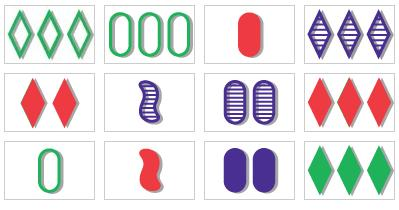
\includegraphics{figures/set_game.jpg}

\vspace{5mm}

This collection of cards contains 5 unique sets:
\vspace{5mm}

\begin{figure}[H] % Briefly describe the figure.
\captionsetup[subfigure]{justification=centering}
\centering
\begin{subfigure}{.47\textwidth}
    \centering
    
\includegraphics[width=\linewidth]{figures/set1.jpg}
    \caption{Same in quantity and shape; different in pattern and color}
    \label{fig:labelthefirstfigure}
\end{subfigure}
\begin{subfigure}{.47\textwidth}
    \centering
    
\includegraphics[width=\linewidth]{figures/set2.jpg}
    \caption{Same in pattern; different in shape, quantity and color}
    \label{fig:labeltheotherfigure}
\end{subfigure}%
\begin{subfigure}{.47\textwidth}
    \centering
    
\includegraphics[width=\linewidth]{figures/set3.jpg}
    \caption{Same in shape; different in quantity, pattern and color}
    \label{fig:labeltheotherfigure}
\end{subfigure}
\begin{subfigure}{.47\textwidth}
    \centering
    
\includegraphics[width=\linewidth]{figures/set4.jpg}
    \caption{Different in all aspects}
    \label{fig:labeltheotherfigure}
\end{subfigure}
\begin{subfigure}{.47\textwidth}
    \centering
    
\includegraphics[width=\linewidth]{figures/set5.jpg}
    \caption{Different in all aspects}
    \label{fig:labeltheotherfigure}
\end{subfigure}
\caption{Five unique sets from the above group of cards}
\end{figure}

\vspace{5mm}

Use the principles of Test Driven Development to write a function that takes as input 12 Set cards and returns the number of sets they contain. Begin by writing test cases for your code. Focus on \emph{what} you want to implement rather \emph{how} you are going to implement it. Use these specifications:
\begin{itemize}
\item Each card in Set can be uniquely represented by a 4 bit integer in base 3, where each digit represents a different property and each property has 3 possible values. Represent a group of Set cards as a text file where each line contains a 4 bit number representing one card.
\item Have your program throw an error if the input is invalid (anything that is not a valid Set card as described above),  if a duplicate card is entered, if less or more than 12 cards are given, or if the file name given is not valid.
\item Ensure that each possible error gives an appropriate error message.
\item Aggregate all your text files in a single folder called ``hands" and upload the folder to your git repository along with your code.
\end{itemize}

Consider breaking this problem down into a few smaller functions and writing a unit test for each function.

\end{problem}

\begin{problem}
Now that you have written test cases for a set game pattern recognizer, write code until all your test cases pass. Write this code at the end of \li{solutions.py}. Rather than running this file to see if your code is working, simply run the test file to see if all the test cases pass. Here are some suggestions for writing the implementation:

Hint: Given three integer which represent cards, the cards form a set if their columns each sum to a multiple of 3.

\end{problem}

\section*{Additional Material} %===========================================

\subsection*{Python Debugger} % -----------------------------------------------

Python has a built in debugger called pdb (Python DeBugger) to aid in finding mistakes in code.
Pdb runs in the terminal or in a Jupyter Notebook.

A \emph{break point} is a spot where the program will pause while running.
Setting break points allows you to view the state of your program while it is running.

To begin using pdb, import it in your program:

\begin{lstlisting}
>>> import pdb
\end{lstlisting}

then add

\begin{lstlisting}
... pdb.set_trace()
\end{lstlisting}

where you would like to set a breakpoint.
Then when you run your code, instead of running in its entirety, it will run until it reaches the break point and then the pbd prompt will be displayed, waiting for a command:

\begin{lstlisting}
(Pdb)
\end{lstlisting}

At this point there are several commands you can run, depending on what you want to do.

\begin{table}[H]
\centering
\begin{tabular}{r|l}
    Command & Description\\
    \hline
    \li{n} & ``Next": executes the next line\\
    \li{p <var>} & ``Print": displays the value of the specified variable\\
    \li{c} & ``Continue": Stops debugging and runs the program normally to the end\\
    \li{q} & ``Quit": terminates the program\\
    \li{l} & ``list": shows several lines of code around the current line\\
    \li{r} & ``Return": returns to the end of a subroutine\\
    \li{<Enter>} & Executes the most recent command again
\end{tabular}
\end{table}

\begin{info}
Pdb provides the freedom to change the values of your variables while debugging.
Suppose you are debugging the following code:

\begin{lstlisting}
def func():
    pdb.set_trace()
    foo = 1
    bar = 2
    return foo + bar + 42
\end{lstlisting}

While debugging, you realize that the value of \li{foo} was initialized wrong.
Then after \li{foo} has been initialized you can enter the command

\begin{lstlisting}
(Pdb) foo = 5
\end{lstlisting}
and the value of the variable will be changed as the program continues to run and the program will return 49 instead of 45.
\end{info}
